\documentclass{standalone}
\usepackage{tikz}
\usetikzlibrary{positioning}

\begin{document}

    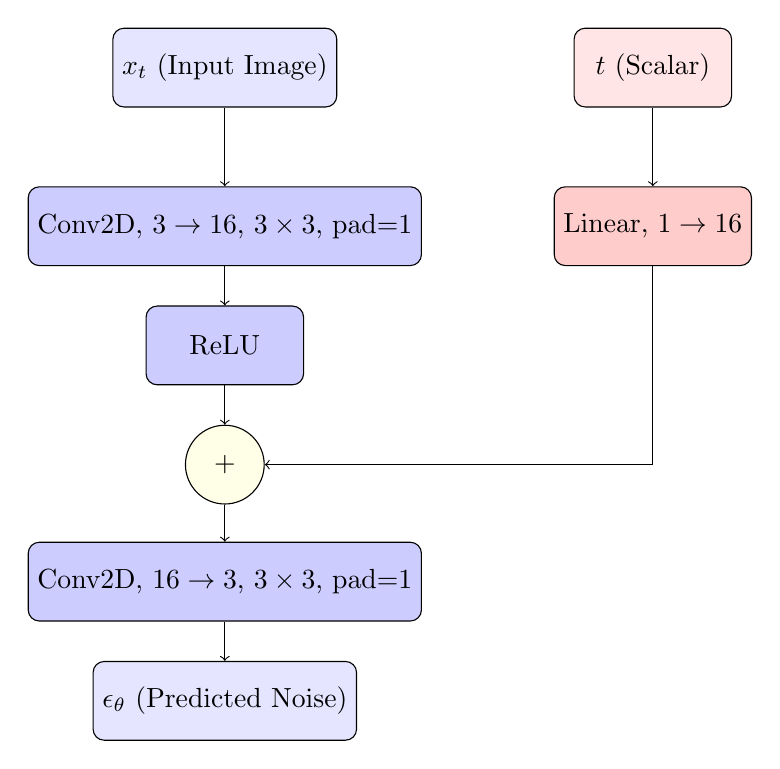
\begin{tikzpicture}

        % Input tensors
        \node[draw, rounded corners, fill=blue!10, minimum width=2cm, minimum height=1cm] (input_x) at (0,0) {$x_t$ (Input Image)};
        \node[draw, rounded corners, fill=red!10, minimum width=2cm, minimum height=1cm, right=3cm of input_x] (input_t) {$t$ (Scalar)};

        % Convolution layers with detailed values
        \node[draw, rounded corners, fill=blue!20, minimum width=3cm, minimum height=1cm, below=1cm of input_x] (conv1) {Conv2D, $3 \to 16$, $3 \times 3$, pad=1};
        \node[draw, rounded corners, fill=blue!20, minimum width=3cm, minimum height=1cm, below=3.5cm of conv1] (conv2) {Conv2D, $16 \to 3$, $3 \times 3$, pad=1};

        % ReLU
        \node[draw, rounded corners, fill=blue!20, minimum width=2cm, minimum height=1cm, below=0.5cm of conv1] (relu) {ReLU};

        % Linear layer
        \node[draw, rounded corners, fill=red!20, minimum width=2cm, minimum height=1cm, below=1cm of input_t] (linear) {Linear, $1 \to 16$};

        % Addition node as a circle with "+"
        \node[draw, circle, fill=yellow!10, minimum width=1cm, minimum height=1cm, below=0.5cm of relu] (add) {+};

        % Output tensor
        \node[draw, rounded corners, fill=blue!10, minimum width=2cm, minimum height=1cm, below=0.5cm of conv2] (output) {$\epsilon_{\theta}$ (Predicted Noise)};

        % Draw connections with right angles
        \draw[->] (input_x) -- (conv1);
        \draw[->] (conv1) -- (relu);
        \draw[->] (input_t) -- (linear);
        \draw[->] (relu) -- (add);
        \draw[->] (linear) |- (add); % Right-angle connection
        \draw[->] (add) -- (conv2);
        \draw[->] (conv2) -- (output);

    \end{tikzpicture}

\end{document}
